\documentclass[tikz,border=2pt]{standalone}
\usepackage{pgfplots}
\pgfplotsset{compat=1.18}

\begin{document}
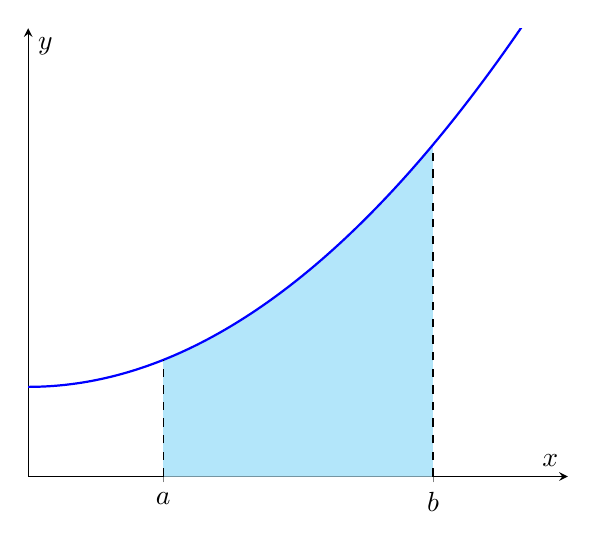
\begin{tikzpicture}
  \begin{axis}[
      axis lines = middle,
      xlabel = {$x$},
      ylabel = {$y$},
      domain = 0:4,
      samples = 100,
      ymin = 0, ymax = 5,
      xmin = 0, xmax = 4,
      xtick = {1, 3},
      xticklabels = {$a$, $b$},
      ytick = \empty
    ]
    \addplot[fill=cyan!30, draw=none, domain=1:3] {0.3*x^2 + 1} \closedcycle;
    \addplot[thick, blue] {0.3*x^2 + 1} node[above right] {$f(x)$};
    \draw[dashed, thin] (axis cs:1,0) -- (axis cs:1,{0.3*(1)^2 + 1});
    \draw[dashed, thin] (axis cs:3,0) -- (axis cs:3,{0.3*(3)^2 + 1});
  \end{axis}
\end{tikzpicture}
\end{document}